% !TeX root = Stageportfolio.tex



\begin{landscape}
	\subsubsection{Les 16-17}
	\begin{tabularx}{1.56\textwidth}{|p{0.35\textwidth}|X|}\hline
		\textbf{Administratieve gegevens}\newline\newline
		Kevin Truyaert\newline\newline
		technisch secundair onderwijs\newline
		3e graad, 1ste jaar, Techniek-Wetenschappen\newline
		VVKSO: \href{http://ond.vvkso-ict.com/leerplannen/doc/Toegepaste\%20fysica-2014-041.pdf}{http://ond.vvkso-ict.com/leerplannen /doc/Toegepaste\%20fysica-2014-041.pdf} \newline
		\underline{Lesonderwerp}:\newline Magnetische flux, Magnetische fluxverandering, De wet van Faraday \& De wet van Lenz & \textbf{Doelstellingen}
		\begin{itemize}[itemsep=0.08\baselineskip]
			\item B27: Fluxverandering als oorzaak van inductiespanning toelichten
			\item B28: Met behulp van de wet van Lenz de zin van de inductiespanning vinden
		\end{itemize}
		\underline{Lesdoelen}\newline
		\vspace{-0.75cm}
		\begin{enumerate}[itemsep=0.08\baselineskip]
			\item De leerlingen begrijpen conceptueel wat de magnetische flux is.
			\item De leerlingen kennen de drie factoren die de magnetische flux bepalen.
			\item De leerlingen kunnen de magnetische flux berekenen.
			\item De leerlingen begrijpen hoe een fluxverandering kan ontstaan.
			\item De leerlingen kunnen de fluxverandering berekenen.
			\item De leerlingen ervaren het ontstaan van een inductiespanning door middel van een fluxverandering via demo's.
			\item De leerlingen ervaren de analogie tussen elektriciteit en magnetisme bij het bespreken van inductieverschijnselen.
			\item De leerlingen kunnen de wet van Faraday zelf, via een demo, samenstellen.
			\item De leerlingen kunnen de zin van de inductiestroom bepalen.
			\item De leerlingen kunnen de wet van Lenz verwoorden.
		\end{enumerate} \\\hline
	\end{tabularx}\vfill \textcolor{white}{.} 


	\begin{tabularx}{1.56\textwidth}{|p{0.55\textwidth}|X|}
		\hline
		\multirow{2}{0.55\textwidth}{\textbf{Beginsituatie}\newline  
		Er zijn acht leerlingen binnen 5TW. Er heerst een algemene tot positieve klassfeer. De leerlingen hebben al theorie gekregen  rond en oefeningen gemaakt op de magnetische krachtwerking. \newline\newline De leerlingen hebben de dag hiervoor hun labo over de lorentzkracht ingediend. Tijdens de lessen fysica die de leerkracht verzorgt, gaat het al een tijdje over kinematica. De leerlingen zijn dus wel nog wat vertrouwt met magnetisme (labo), maar zien ook andere fysica. Eventueel zou hierdoor wat verwarring kunnen ontstaan. \newline\newline Deze les omvat een volledig nieuw stuk theorie. Nieuwe theorie is voor mij een valkuil om in doceermodus te gaan. Ik wil mij hiervan bewust zijn en hier op letten om meer vraag gesteld les te geven en over te gaan op een onderwijsleergesprek-modus.} & \textbf{Acties}\newline\newline  
		- Magnetische flux is een concept dat niet voor te stellen valt. De gevolgen van deze flux kan je wel voorstellen en worden uitvoerig in hoofdstuk 6 besproken. Vooraleer je deze concepten echter kan beginnen te bespreken, moeten de leerlingen de basis van elektromagnetische inductie beheersen, waarvoor ze magnetische flux(verandering) moeten begrijpen. Toch verwacht ik dat de leerlingen hier vlot mee weg zullen zijn en wil ik veel in interactie treden met de leerlingen. \newline\newline
		- \GreenHighlight{Via demo's wil ik bepaalde onderwerpen starten.}{9cm}	Op die manier kan ik de interesse van de leerlingen wekken en kan ik fysische wetmatigheden hen effectief aantonen. Zo kunnen leerlingen op een klassikale manier zelfstandig dingen ontdekken.	
		\newline\newline\newline\newline
		
		\\ \cline{2-2}
		  & \textbf{Bronnen}\begin{itemize}
		  	\item Schramme, S. (2018-2019) Cursus hoofdstuk 5: elektromagnetische inductie
		  	\item Giancoli, D. C. (2008). Physics for scientists and engineers. Pearson Education International.
		  \end{itemize}\\ \hline
	\end{tabularx}


\newpage
	

\begin{tabularx}{1.56\textwidth}{|p{1.5cm}|p{9cm}|X|p{4cm}|}
	\hline
	\textbf{Nr. lesdoel } & \textbf{Inhoud (timing)}  & \textbf{Organisatie } & \textbf{Media } \\ \hline
	 1\newline\newline 2&\underline{Introductie magnetisme hoofdstuk 5:  } \underline{ Elektromagnetische inductie:} \underline{de magnetische flux (10 minuten)}\newline
	Het concept van magnetische flux wordt ingeleid, samen met de drie componenten waaruit die bestaat. We bespreken klassikaal de eigenschappen
	&  \underline{Onderwijsleergesprek}\newline 
	Ik teken de situatie zoals op pagina 1 van hoofdstuk 5 op het bord en stel gerichte vragen aan de leerlingen zodat zij de concretere eigenschappen van de situatie verwoorden (Hoe liggen de polen?, hoe ligt de hoek $\alpha$? \ldots). Wat gebeurt er als we nu enkele dingen aanpassen? Welke parameters kunnen we aanpassen om een andere flux te bekomen?	De uiteindelijke vergelijking ($\Phi = BA\cos(\alpha)$) blijft met de tekening op het linkerbord staan. De eenheid van flux wordt ook benoemd.
	&  Cursus hoofdstuk 5 pagina 1,2\newline\newline Krijtbord
	\\ \hline
\end{tabularx}

\begin{tabularx}{1.56\textwidth}{|p{1.5cm}|p{8cm}|X|p{3cm}|}
	\hline
	\textbf{Nr. lesdoel } & \textbf{Inhoud (timing)}  & \textbf{Organisatie } & \textbf{Media } \\ \hline
	3& \underline{Magnetische flux: Oefeningen (15 minuten)}\newline
	Aangezien de leerlingen net de eigenschappen van magnetische flux gezien hebben, maken we eerst wat oefeningen hierop. Zo kunnen de leerlingen een beter begrip hierover krijgen.
	&  \underline{Onderwijsleergesprek + oefeningen}\newline  Oefening 2 a en b maak ik klassikaal met de leerlingen samen. Hierna werken de leerlingen oefening 2 individueel af. Ik schrijf ook op bord dat de leerlingen verder kunnen gaan met oefeningen 4, 5 en 6. De eindoplossing van die oefeningen komen op bord, de werkwijze zal enkel van oefening 5 op bord komen indien nodig, gezien die wat moeilijker is.
	&  Cursus hoofdstuk 5 p4-5\newline\newline Krijtbord
	\\ \hline
\end{tabularx}\vspace{5mm}


\begin{tabularx}{1.56\textwidth}{|p{1.5cm}|p{8cm}|X|p{3cm}|}
\hline
\textbf{Nr. lesdoel } & \textbf{Inhoud (timing)}  & \textbf{Organisatie } & \textbf{Media } \\ \hline
4& \underline{Magnetische fluxverandering:} \underline{theorie (15 minuten)}\newline
Aangezien de leerlingen net de eigenschappen van magnetische flux gezien hebben, definieer ik nu de magnetische fluxverandering. De leerlingen komen te weten hoe die verandering tot stand kan komen.
&  \underline{Onderwijsleergesprek}\newline 
Ik teken een situatie met een magnetische flux op bord en de leerlingen zeggen mij wat de belangrijke eigenschappen zijn in verband met magnetische flux. Ik vraag de leerlingen hoe die fluxverandering kan ontstaan (net vanuit één van die drie eigenschappen). Zo bespreken we alle mogelijkheden van de opwekking van een fluxverandering.	
&  Cursus hoofdstuk 5 p2-3\newline\newline Krijtbord
\\ \hline
\end{tabularx}\vspace{5mm}



\begin{tabularx}{1.56\textwidth}{|p{1.5cm}|p{8cm}|X|p{3cm}|}
	\hline
	\textbf{Nr. lesdoel } & \textbf{Inhoud (timing)}  & \textbf{Organisatie } & \textbf{Media } \\ \hline
	4\newline\newline 5& \underline{Magnetische fluxverandering:} \underline{Oefeningen (13 minuten)}\newline
	Aangezien de leerlingen net de eigenschappen van magnetische fluxverandering gezien hebben, maken we eerst wat oefeningen hierop, om een beter begrip van de fluxverandering te krijgen. Dat is essentieel om aan inductiespanning te kunnen beginnen.
	&  \underline{Onderwijsleergesprek + oefeningen}\newline  Oefening 7 maak ik klassikaal, met de leerlingen samen, via vraagstelling aan de leerlingen. Hierna werken de leerlingen individueel oefening 8 en 9. Ik schrijf enkel de tussenoplossingen en de eindoplossing op bord. 
	&  Cursus hoofdstuk 5 p5-6\newline\newline Krijtbord
	\\ \hline
\end{tabularx}\vspace{5mm}


\begin{tabularx}{1.56\textwidth}{|p{1.5cm}|p{8cm}|X|p{3cm}|}
\hline
\textbf{Nr. lesdoel } & \textbf{Inhoud (timing)}  & \textbf{Organisatie } & \textbf{Media } \\ \hline
& \underline{Pauze (2 minuten)}\newline
Even uitblazen tijdens het blokuur
&  \underline{Pauze}\newline 
Ik plaats het materiaal voor de demo rond inductiespanning en -stroom op tafel.
&  Cursus hoofdstuk 5 p5-6\newline\newline Krijtbord
\\ \hline
\end{tabularx}\vspace{5mm}



\begin{tabularx}{1.56\textwidth}{|p{1.5cm}|p{9cm}|X|p{4cm}|}
	\hline
	\textbf{Nr. lesdoel } & \textbf{Inhoud (timing)}  & \textbf{Organisatie } & \textbf{Media } \\ \hline
	6\newline\newline 7& \underline{Inductiespanning en -stroom:} \underline{Inleiding (10 minuten)}\newline
	Er werd in vorige lessen (Hoofdstuk 2) door de leerlingen ondervonden dat een elektrische stroom een magnetisch veld veroorzaakt. Hier onderzoeken we of het omgekeerde ook waar is: induceert een magnetisch veld een elektrische stroom in een gesloten circuit? Dit zal een interactie tussen elektriciteit en magnetisme aan de leerlingen tonen.
	&  \underline{Demonstratie + Onderwijsleergesprek}\newline 
	Ik begin de les met een applicatie van Walter Fendt die aantoont dat een magnetisch veld door een stroomgeleidende draad kan ontstaan. Hier vraag ik aan de leerlingen wat zij zien. Daarna vertel ik hen dat we gaan onderzoeken of het omgekeerde ook waar is.\newline De opstelling bestaat uit een spoel die aangesloten is aan een milliampèremeter, die zowel negatieve als positieve stromen kan meten. Daarna beweeg ik een magneet naar de spoel. Ik zeg niets en vraag aan de leerlingen wat zij beschrijven wat er gebeurt. Hier speel ik op in en treed ik in interactie met de leerlingen om van hen te horen wat zij ervaren wat er gebeurt.	Op basis hiervan interageer ik met de leerlingen om hen in hun bewoording te begeleiden. Hierna vullen we samen op basis van de demo pagina's 7 en 8 in.
	&  Cursus hoofdstuk 5 p7-8\newline\newline Krijtbord\newline\newline App (\href{https://www.walter-fendt.de/html5/phnl/magneticfieldwire_nl.htm}{Link App})
	\\ \hline
\end{tabularx}\vspace{5mm}




\begin{tabularx}{1.56\textwidth}{|p{1.5cm}|p{9cm}|X|p{4cm}|}
	\hline
	\textbf{Nr. lesdoel } & \textbf{Inhoud (timing)}  & \textbf{Organisatie } & \textbf{Media } \\ \hline
	7\newline\newline 8& \underline{De wet van Faraday:} \underline{Verbanden (15 minuten)}\newline
	Er is nu aangetoond dat in een gesloten circuit er een inductie stroom is. Maar eigenlijk ontstaat er een inductiespanning en is de stroom een gevolg van dat geïnduceerd spanningsverschil. Hieruit is het mogelijk om de inductiespanning te meten door middel van een fluxverandering. Door verschillende wijzigingen aan de situatie toe te brengen, kunnen de leerlingen zelf bepaalde evenredigheden uit de demonstratie halen. Samen met de leerlingen leid ik de wet van Faraday af.
	&  \underline{Demonstratie + Onderwijsleergesprek}\newline 
	De opstelling bestaat uit een spoel die aangesloten is aan een voltagemeter, die zowel negatieve als positieve spanningen kan meten. Daarna beweeg ik een magneet naar de spoel. Ik zeg niets en vraag aan de leerlingen wat zij beschrijven wat er gebeurt. Hier speel ik op in en treed ik in interactie met de leerlingen om van hen te horen wat zij ervaren wat er gebeurt.	Deze resultaten zullen ze snel begrijpen, gezien we net de situatie van de inductiestroom gezien hebben. Nu verander ik de windingen van de spoel, de flux (door middel van de magneet) en de tijdspanne waarin ik de magneet dichter breng. Deze relaties leiden uiteindelijk tot de wet van Faraday. Hierna vullen we samen op basis van de demo pagina's 9 en 10 in. 
	&  Cursus hoofdstuk 5 p9-10\newline\newline Krijtbord
	\\ \hline
\end{tabularx}\vspace{5mm}


\begin{tabularx}{1.56\textwidth}{|p{1.5cm}|p{8cm}|X|p{4cm}|}
	\hline
	\textbf{Nr. lesdoel } & \textbf{Inhoud (timing)}  & \textbf{Organisatie } & \textbf{Media } \\ \hline
	9\newline\newline 10&\underline{De wet van Lenz (19 minuten)}\newline
	De leerlingen bepalen de zin van de inductiestroom  aan de hand van een demo.
	&  \underline{Demo + Onderwijsleergesprek}\newline 
	Door middel van een elektromagneet (i.e. een spoel met een weekijzeren kern), wordt een stroom  in een ring, die rond de weekijzeren kern hangt, geïnduceerd. De leerlingen zullen die zien bewegen op het moment dat de kring gesloten wordt en terug geopend wordt. Samen leiden we af hoe de inductiestroom loopt, op basis van de beweging van de ring t.o.v. het magnetisch veld van de spoel. Zo worden pagina's 11 en 12 in de bundel aangevuld, aan de hand van wat de leerlingen observeren wat er met de ring gebeurt. Daarna besluiten we met de definitie van de wet van Lenz. Ik probeer de leerlingen deze eens in eigen woorden ook zeggen, omdat dit een belangrijk gegeven is voor de toepassingen die in hoofdstuk 6 aan bod komen. 
	&   Cursus hoofdstuk 5 p11-12\newline\newline Krijtbord \newline\newline Elekromagneet, weekijzeren kern, hangende ring
	\\ \hline
\end{tabularx}\vspace{5mm}

\begin{tabularx}{1.56\textwidth}{|p{1.5cm}|p{9cm}|X|p{4cm}|}
	\hline
	\textbf{Nr. lesdoel } & \textbf{Inhoud (timing)}  & \textbf{Organisatie } & \textbf{Media } \\ \hline
	& \underline{Slot (1 minuut)}\newline
	Ik herhaal nog even kort samen met de leerlingen de wet van Faraday en van Lenz. 
	&  \underline{Vertellen}\newline 
	Bespreken van de wet van Faraday en fluxverandering
	&  
	\\ \hline
\end{tabularx}




	
\end{landscape}


%\subsection*{Bijlage 5.1: slides introductie}

%
%\subsection*{Bijlage 1.2: bordschema theorie}
%\begin{center}
%	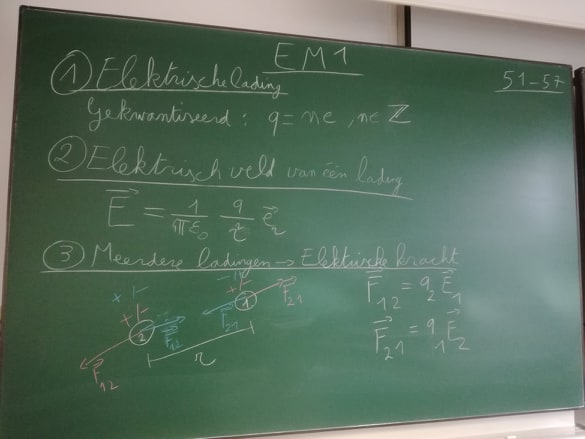
\includegraphics[width=0.9\textwidth]{Bord1a}
%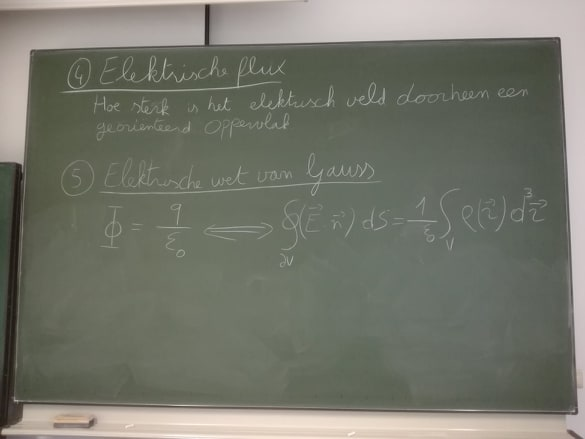
\includegraphics[width=0.9\textwidth]{Bord1b}
%\end{center}
%\newpage
%
%
%\includepdf[scale = 0.8,pages = 17,pagecommand=\subsection*{Bijlage 1.3: opgeloste oefeningen}]{Observaties_OpgelosteOef}
%\includepdf[scale = 0.8,pages =18-20,pagecommand=]{Observaties_OpgelosteOef}
%
%
%
%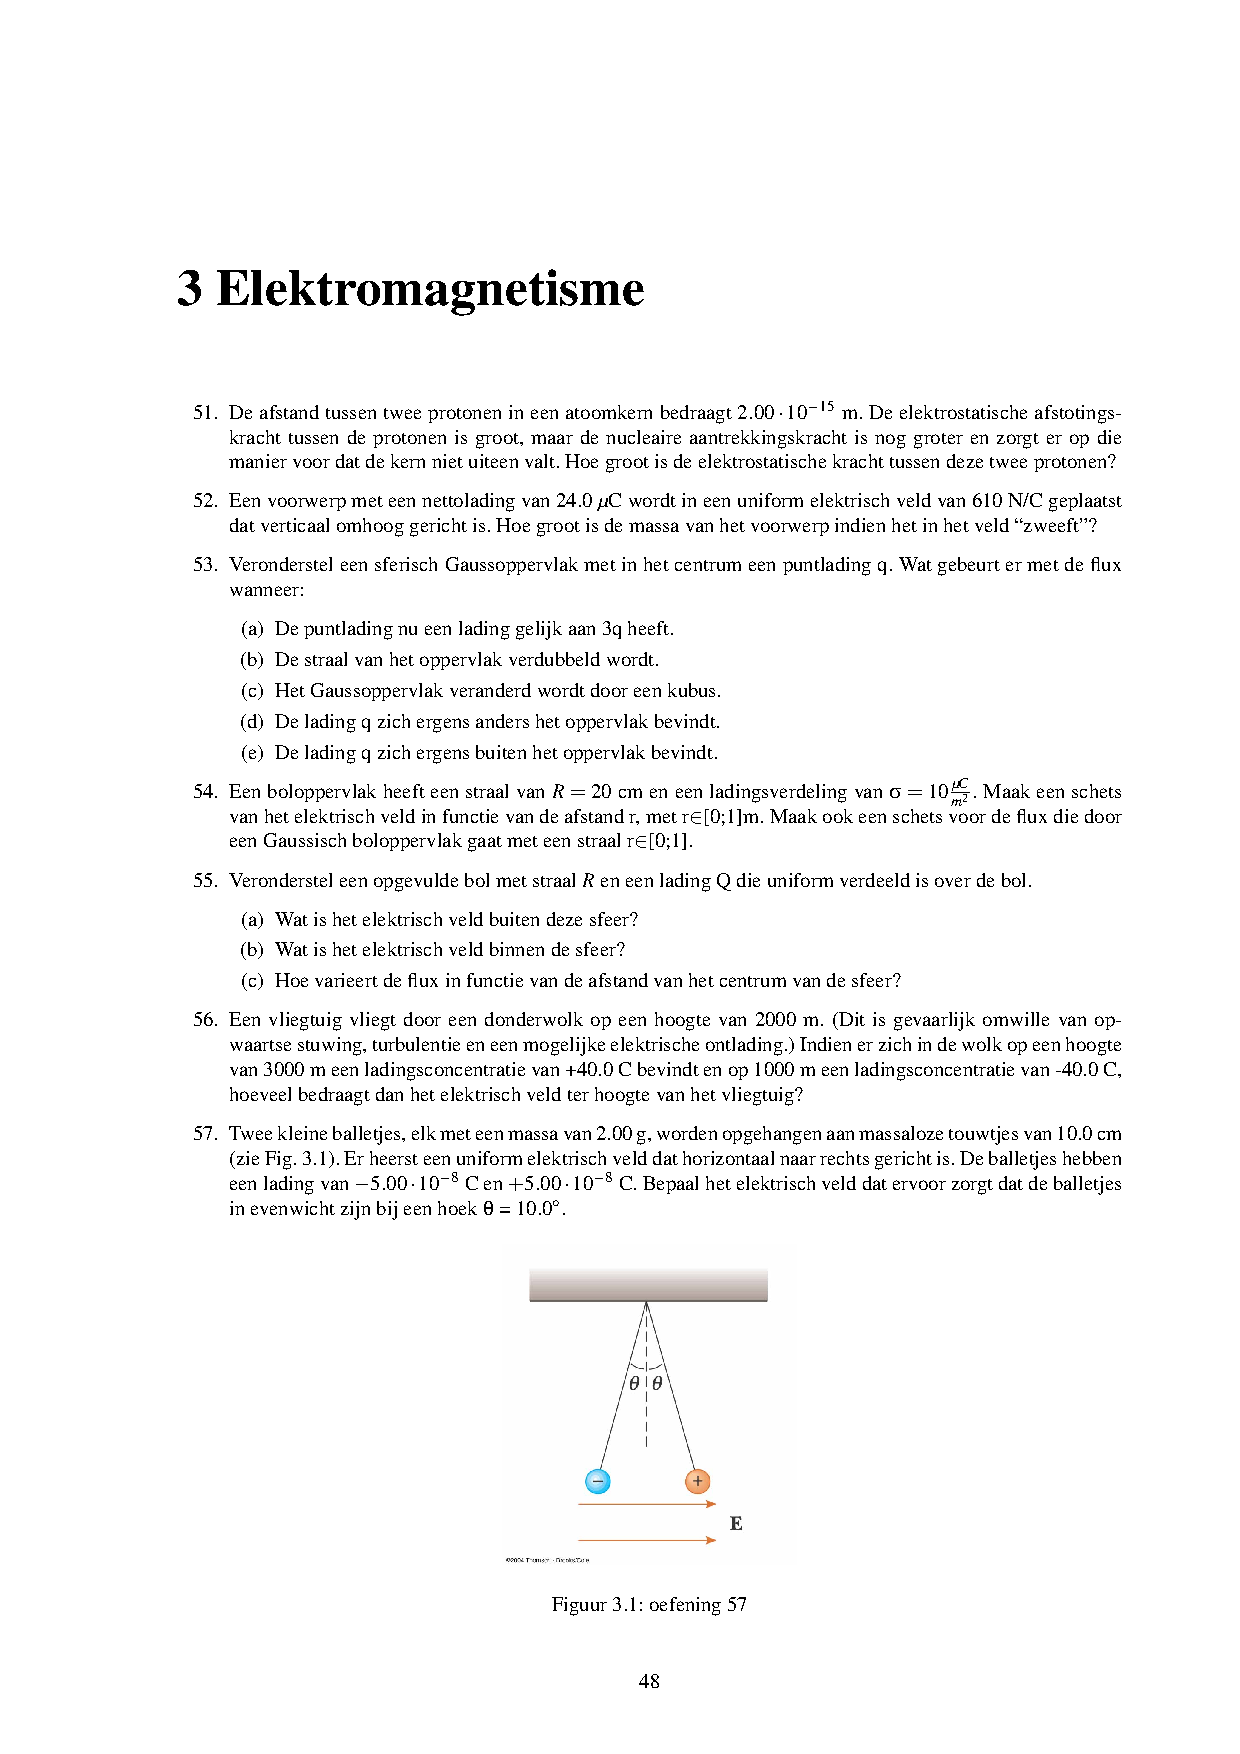
\includepdf[scale = 0.95,pages = 1,pagecommand=\subsection*{Bijlage 1.4: oefeningenbundel elektromagnetisme}]{OefeningenBundel}
%\includepdf[scale = 0.95,pages =2-,pagecommand=]{OefeningenBundel}